 \subsubsection{Passive 2-Tore} \label{subsubsec:2tore}
 Folgendes Kapitel basiert auf der Quelle \cite{p._niklaus_2-tore_2019} Passive 2-Tore sind Netzwerke mit 2 Klemmenpaaren, die in jedem Betriebszustand Leistung verbrauchen. Ein Klemmenpaar wird auch als Tor bezeichnet. Dabei wird ein Tor als Eingang für ein elektrisches Signal verwendet. Folglich wird am anderen Tor das Ausgangssignal abgegriffen. Ein Netzwerk, das intern nur aus beliebigen R-(ohmischer Widerstand), L-(Induktivität), C-(Kapazität) und M-(Gegeninduktivität) Komponenten aufgebaut ist, ist immer ein passives Netzwerk. Ein solches 2-Tor ist in der Abbildung \ref{fig:tor2} dargestellt.

\begin{figure}[H]
	\centering
	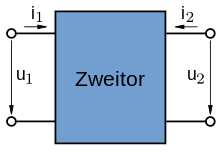
\includegraphics[width=8cm]{2Tor.png}
	\caption{Zweitor (2-Tor) \cite{p._niklaus_2-tore_2019} }
	\label{fig:tor2}
\end{figure}

Ein solches Netzwerk ist zusätzlich noch reziprok. Reziproke Netzwerke haben die Eigenschaft, dass es egal ist, in welche Richtung sie betrieben werden, solange der Innenwiderstand der Quelle gleich gross wie die Lastimpedanz ist. Anhand vom folgenden Beispiel (Abbildung: \ref{fig:bsp_reziprok}) wird dies veranschaulicht. Die Leistung im Verbraucher ist in beiden Betriebszuständen dieselbe. Mit dieser Eigenschaft können in der  Praxis die Berechnungen sehr vereinfacht werden. 

\begin{figure}[H]
	\centering
	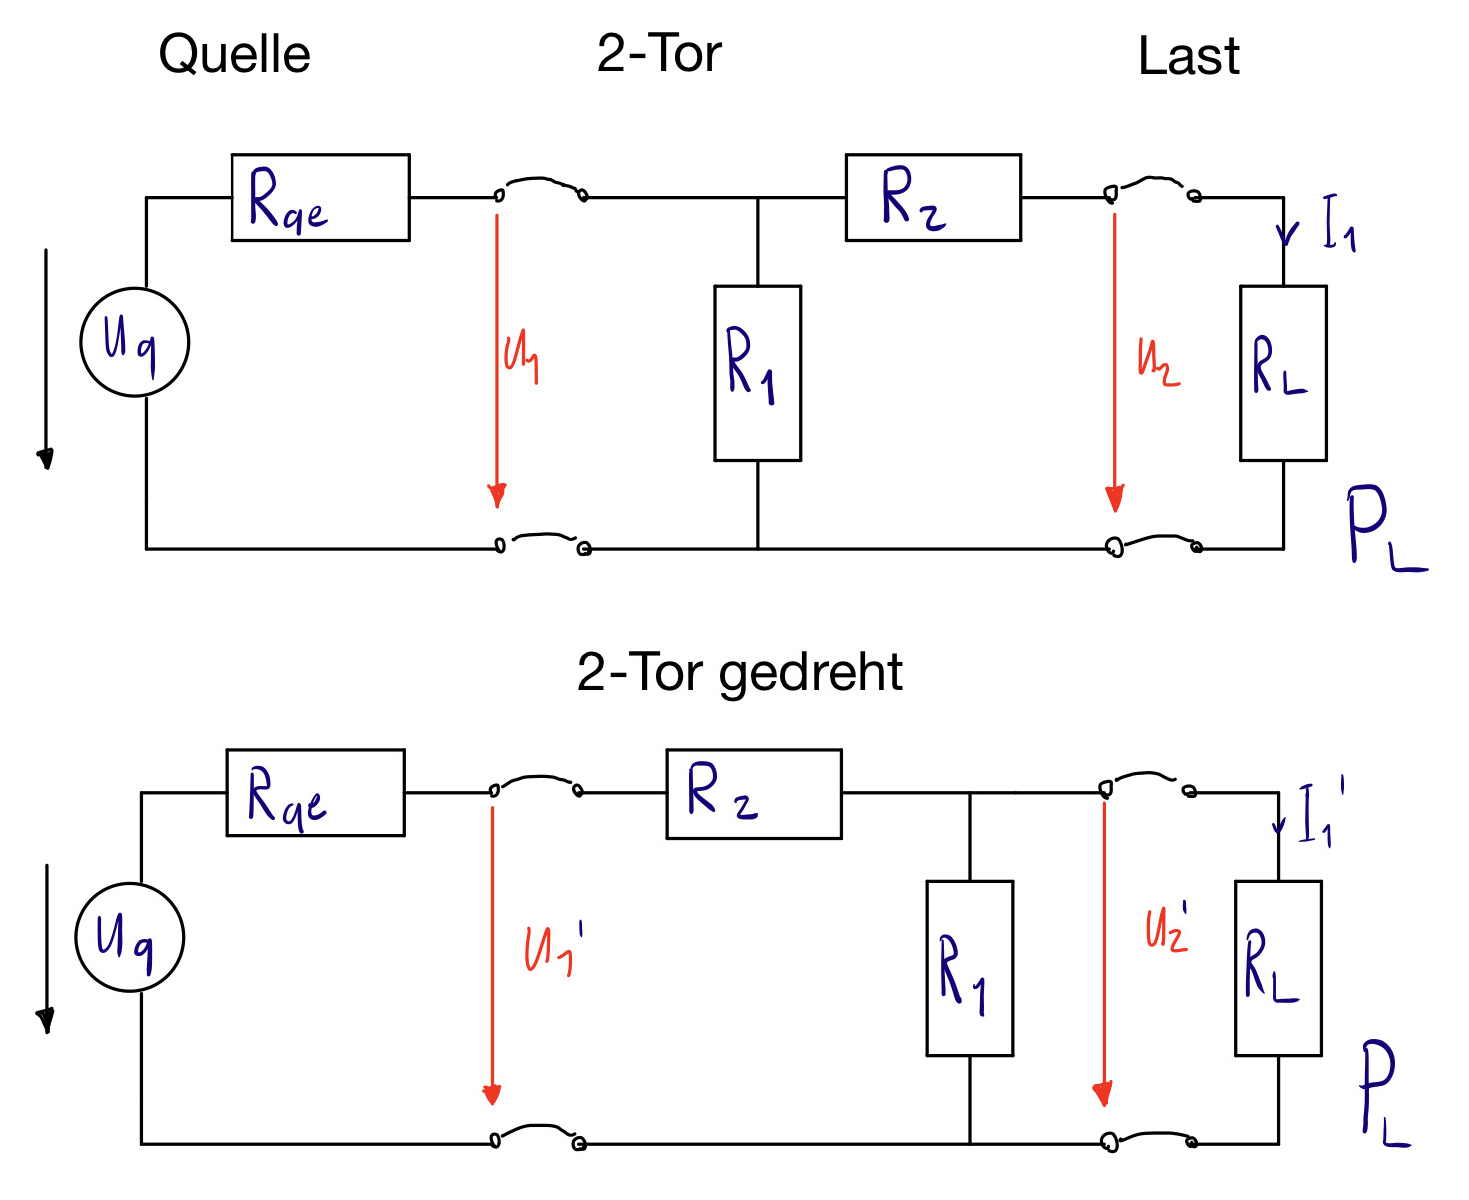
\includegraphics[width=10cm]{bsp_reziprok.png}
	\caption{Beispiel Reziprozitat}
	\label{fig:bsp_reziprok}
\end{figure}


Als Beispiel sind R$_qe$ und R$_L$ jeweils 50 Ohm, R$_1$ 150 Ohm und R$_2$ 20 Ohm. Die Quelle hat eine Spannung von 100V.

In beiden Netzwerken werden jeweils aus der Quelle und dem 2-Tor der Ersatzwiderstand  R$_q1$ und R$_q2$ berechnet.

\begin{equation}\label{equ:rqe1}
			R_{q1} = \frac{1}{\frac{1}{R_Q+R_2}+\frac{1}{R_1}} =  47.73 \Omega 
		\end{equation}
		
\begin{equation}\label{equ:rqe2}
			R_{q2} = \frac{1}{\frac{1}{R_Q}+\frac{1}{R_1}} +R_2 =  57.5 \Omega 
		\end{equation}

Aus dem Ersatzwiderstand berechnen wir den Gesamtstrom in beiden Schaltungen. 

\begin{equation}\label{equ:itot1}
    I_{tot1} = \frac{U_{q}}{R_{q1}} =  1.02A 
  \end{equation}
  
\begin{equation}\label{equ:itot2}
    I_{tot2} = \frac{U_{q}}{R_{q2}} =  0.93A 
  \end{equation}		
  
 Die Spannungen U$_1$ und U$_1'$ sind unterschiedlich und werden per Spannungsteiler bestimmt. 

\begin{equation}\label{equ:u1}
    U_{1} = \frac{U_{q}*R_{q1}}{R_{q1}+R_{qe}} =  48.84V
  \end{equation}

\begin{equation}\label{equ:u1'}
    U_{1}' = \frac{U_{q}*R_{q2}}{R_{q2}+R_{qe}} =  53.48V
  \end{equation}


Auf der anderen Seite des Netzwerks hingegen bleiben die Spannungen gleich wie man an den Berechnungen sieht.


\begin{equation}\label{equ:u2}
    U_{2} = \frac{U_{1}\cdot{R_{L}}}{R_{L}+R_{2}} =  34.88V
  \end{equation}

\begin{equation}\label{equ:u2'}
    U_{2}' = \frac{U_{2}\cdot{{ \frac{1}{\frac{1}{R_L}+\frac{1}{R_1}}}}}{{{ \frac{1}{\frac{1}{R_L}+\frac{1}{R_1}}}}+R_2} =  34.88V
  \end{equation}
  
Beim Strom verhält es sich durch den Stromteiler gleich

  \begin{equation}\label{equ:u1}
    I_{1} = \frac{ I_{tot1}\cdot \frac{1}{\frac{1}{R_L+R_2}+\frac{1}{R_1}}}{R_{2}+R_{L}} =  0.69A
  \end{equation}
  
    \begin{equation}\label{equ:u1}
    I_{1}' = \frac{I_{tot2} \cdot \frac{1}{\frac{1}{R_L}+\frac{1}{R_1}}}{R_{L}} =  0.69A
  \end{equation}
  
  
  Dadurch ist auch die Leistung P$_L$ in beiden Fällen gleichgross
  
      \begin{equation}\label{equ:u1}
   P_{L} = U_{2} \cdot I_{1} =  23.3W
  \end{equation}
  

Im dargestellten Netzwerk \ref{fig:beweis} gilt somit

\begin{equation}\label{equ:verticImpedance}
    \underline{I}_b =  \underline{\tilde{I}}_b
  \end{equation}
  
sowie 		
  
\begin{equation}\label{equ:verticImpedance}
    \underline{U}_b =  \underline{\widetilde{U}}_b
  \end{equation}
  
  
  
\begin{figure}[H]
\centering
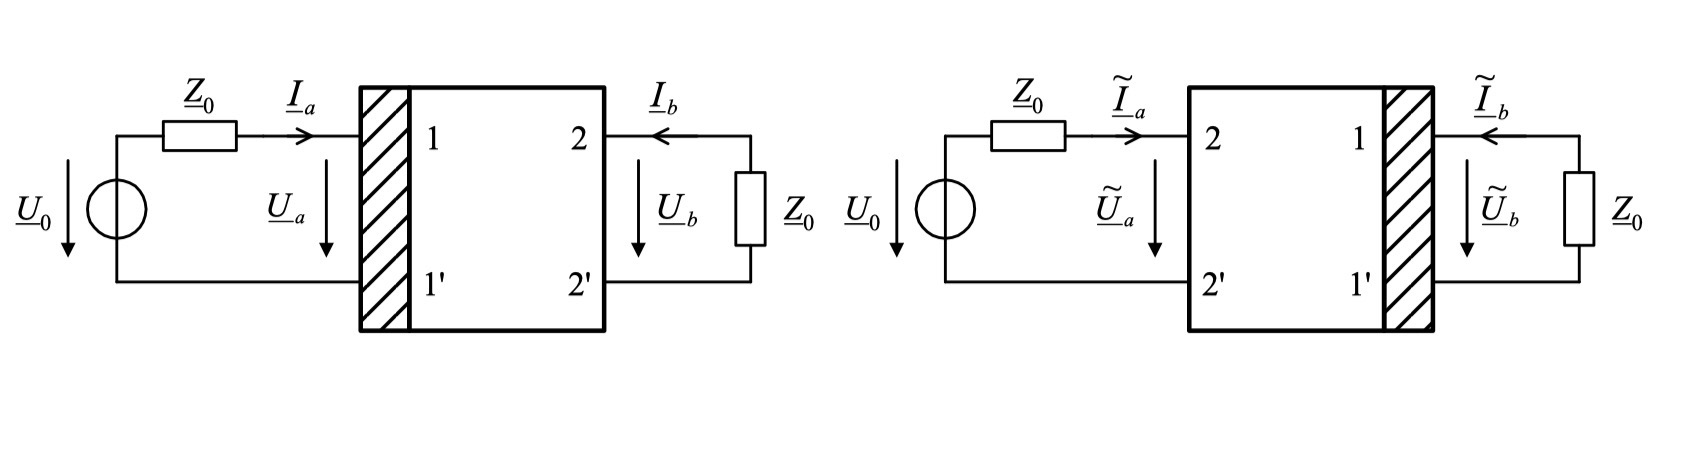
\includegraphics[width=12cm]{reziprozitat.jpg}
	\caption{Reziprozität \cite{p._niklaus_2-tore_2019}}
		\label{fig:beweis}
\end{figure}


\newpage


